\section{Testing Methodology}
The testing and verification of the directional audio system will be done by comparing its acoustic performance with a traditional loudspeaker. Particular test points of interest include the directionality of the speaker and the audible harmonic distortion for pure tone cases.
\subsection{Test setup and apparatus}
The test setup for recording results from both the traditional and ultrasonic directional speaker involves the items shown in table \ref{tab:apparatus}.
\begin{table}[H]
    \centering
    \begin{tabular}{|l|p{12cm}|}
    \hline
         \textbf{Item name}& \textbf{Function} \\ \hline
        Tripod & Stable platform to pan the speaker through a consistent arc \\ \hline
        Microphone & Rhode NT1 Cardioid condenser microphone provides a flat frequency response with a front facing cardioidal recording beam pattern. \\ \hline
        ADC & Focusrite Scarlett 8i6 audio interface provides a 24 bit recording at 44.1 kHz sample rate.\\ \hline
        Recording software & Abelton Live version 10.1.15 used to capture and edit the recording. \\ \hline
        Laptop/Julia & A laptop running Julia version 1.3.1 produces the processed and unprocessed audio. \\ \hline
        Signal generator & Produces the 40 kHz carrier wave \\ \hline
        Mixer & Mixes the baseband audio with the 40kHz carrier to produce AM signal for ultrasonic speaker. \\ \hline
        Power amplifier & Amplifies the signal to $\pm 26 V_{p-p}$ and supplies sufficient power to drive the ultrasonic transducer array.\\ \hline
        Ultrasonic array & This is the constructed ultrasonic array which will emit the directional audio beam. \\ \hline
        Traditional speaker & A regular loudspeaker taking in only baseband audio from the laptop. \\ \hline
    \end{tabular}
    \caption{Table of apparatus used during testing}
    \label{tab:apparatus}
\end{table}
These items were placed in a room with 1.75m separating the centre of the ultrasonic / traditional speaker from the microphone. Figure \ref{fig:testsetup} shows the top down representation of the test setup in a square room. Ideally the test should be done in a larger room with less reflective surfaces; however, due to the Covid-19 pandemic testing resources were limited to what was available at home.

\begin{figure}[ht!]
    \centering
    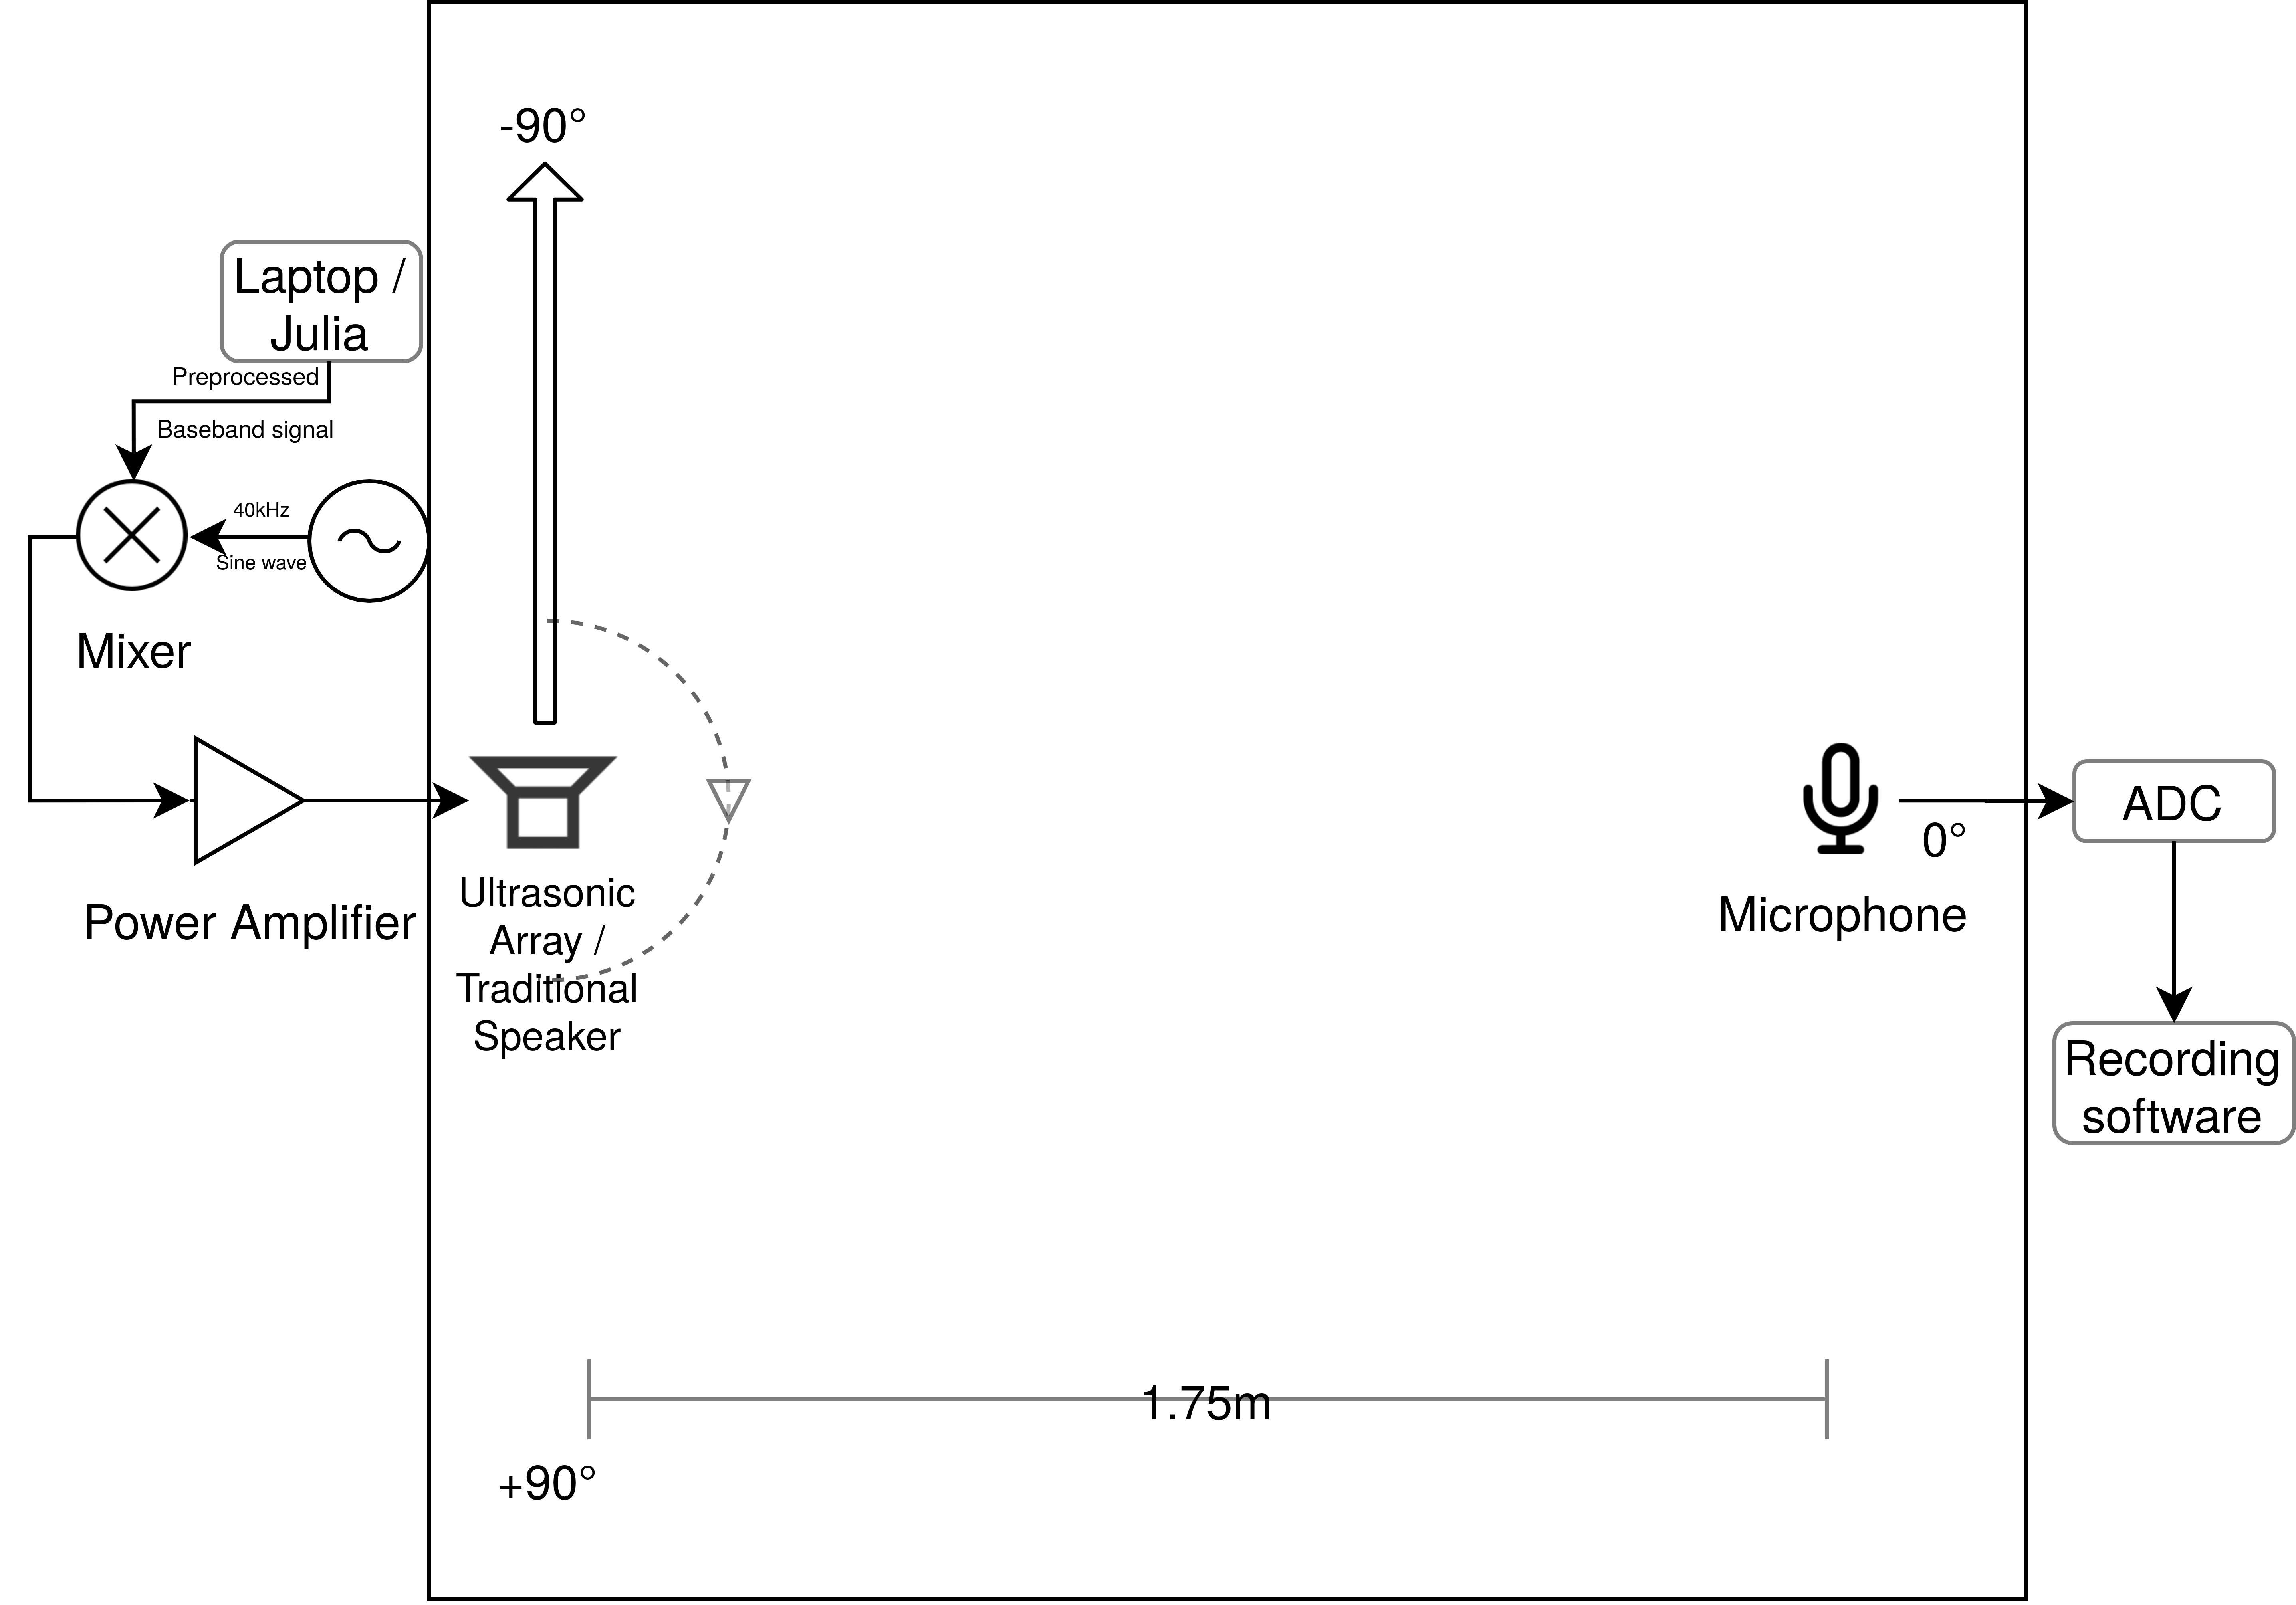
\includegraphics[width=0.8\textwidth]{Figures/Testing/Test_setup.png}
    \caption{The test setup used for distortion and directionality testing.}
    \label{fig:testsetup}
\end{figure}
\newpage
\subsection{Distortion testing method}
To test distortion, the ultrasonic array is directed  $0^\circ$ relative to the microphone (head on) and both a pre-processed and unprocessed 2.5 kHz sine wave are generated in julia, modulated by the mixer and emitted with the array in two separate recordings. One recording for only pre-processed audio and one for no processing and only amplitude modulation.\\
The ultrasonic array is then removed from the tripod and replaced with a traditional speaker. With the speaker facing the same direction as before and using julia on the laptop, a 2.5 kHz sine wave is generated and played by the speaker without any modulation or processing done on the waveform.
Each recording is captured for 15 seconds and edited to only include the period where the signal is audible and no other sources of noise are visible in the waveform.\\
These recordings are then imported into julia and analysed. For each recording, the FFT of the recording is produced to analyse the fundamental frequency magnitude relative to its harmonics. This provides a measure to determine how distorted the output of the speaker is by comparing how close the magnitude of the harmonics is to the fundamental frequency.

\newpage

\subsection{Directionality testing method}
To test directionality, the ultrasonic array is initially directed to $-90^\circ$ relative to the microphone and the pre-processed 2.5kHz sine wave is generated using julia, modulated with the mixer and emitted from the array. A operator then positions themselves behind the tripod and slowly pans the speaker from $-90^\circ$ through $0^\circ$ and finally ending at $+90^\circ$. The recording is then stopped and edited to only include the period over which the array is swept to reduce operator noise affecting the results.\\
A similar method is followed for the traditional speaker directionality test. Beginning at $-90^\circ$, a 2.5kHz sine wave is created in julia and played by the speaker. The same beam sweep method occurs as in the ultrasonic array case and the recording is stopped at the end of the sweep.\\
The recordings are edited to only include the period of the beam sweeping and thus, should produce a maximum near the middle of the recorded time. The FFT for the whole spectrum of the samples is then generated along with the time domain representation of the recorded signal to provide context to what is actually heard during the beam sweep by the microphone.\\
The recordings are then filtered by use of a band-pass FIR filter in the frequency domain using julia with a bandwidth of 100 Hz. The band-pass filter is then centred on the fundamental frequency (2.5 kHz), the first harmonic (5 kHz) and the second harmonic (7.5 kHz) and the time domain representations of the filtered outputs are plotted.\\
The filtering provides a higher signal to noise ratio for the testing signals, thus providing a clearer representation in the time domain of each of these frequencies and how intense they are over the period of the sweep. The time domain representations should indicate how intense each of these frequencies are, especially as they approach the $0^\circ$ angle in the sweep and will produce an approximate beam shape for the directional audio system and the traditional speaker to compare it to.\\
In ideal circumstances, this test could be done with an accurate angle of incidence by using a motor driven platform and recording the signal at set increments in angle. That data could then be used to construct a more accurate beam pattern. This however, was not possible due to restricted access to lab resources as this testing is done during the Covid-19 pandemic. As a result, only an approximate beam shape can be resolved since the angle of incidence is unknown.

%The processes involved in the development of a directional audio system are broken up into %functional deliverables which feed into one another. For this reason a waterfall development %model is used to manage the project development life-cycle.
%\subsection{Theory}
%The theory deliverable involves understanding the various models related to the development of %the directional audio system. This includes understanding the principles behind self-demodulating %ultrasonic waves and how to implement these principles.
%\subsection{Simulation}
%The full signal path is simulated from generation/recording, pre-processing of the signals and %finally to recreation of the medium within which the ultrasonic waves are produced. The %simulations will deliver a flexible environment to test pre-processing ideas and modulation %schemes within some simulation limits. Additionally, the simulations aid in selecting an %appropriate environment to implement the pre-processing while maintaining a low cost.
%\subsection{Design}
%This deliverable aims to create designs of the multiple sub-systems required to produce a %directional audio system. These subsystems include an ultrasonic transducer array, audio signal %pre-processing subsystem, modulation circuit and ultrasonic signal amplifier. Each of these %designs may be iterated upon, thus prototyping and testing of these sub-systems during their %development is expected.
%\subsection{Implementation}
%Implementation of the designs needs to be occur often to test the results of any design changes. %Thus, the designs are prototyped at first on breadboard and stripboard, allowing for flexible %tuning. Upon satisfactory results, the designs may be moved to a full stripboard implementation %and finally if circumstances allow it, a PCB design.
%\subsection{Testing \& Verification}
%The testing and verification of the directional audio system will be done by comparing its %acoustic performance with a traditional loudspeaker. Particular test points of interest include %the directionality of the speaker and the audible harmonic distortion for pure tone cases.

